\documentclass[11pt]{article}

\usepackage[utf8]{inputenc}
\usepackage{graphics}
\usepackage{graphicx}
\usepackage[margin=3cm]{geometry}
\usepackage{placeins}
\usepackage{amsmath}

\usepackage{titlesec}
\usepackage[titles]{tocloft}
\linespread{1.25}
\setlength{\parindent}{0pt}
\setlength{\parskip}{1em}
\titlespacing{\section}{0pt}{\parskip}{-\parskip}
\titlespacing{\subsection}{0pt}{\parskip}{-\parskip}
\titlespacing{\subsubsection}{0pt}{\parskip}{-\parskip} 
\setlength{\cftbeforesecskip}{3pt}
\setlength{\cftbeforesubsecskip}{0pt}
%TODO adjust each of the above values after more text has been filled

\usepackage{hyperref} 
\hypersetup{
    colorlinks   = true,
    urlcolor     = blue,
    linkcolor    = black
}

\title{{\large MSE491 - Application of Machine Learning in Mechatronic Systems} \\ Project Report: \\ Vessel Targeting System for Automated Gantry Robot}
\author{Group 25 \\ Liam Akkerman - 301286906 \\ Aidan Hunter - 301279938}

\begin{document}
    \maketitle
    \vfill
	\setcounter{tocdepth}{2} % only include down to subsections
    \tableofcontents % could move to new page if too long
    \FloatBarrier 
    \newpage

    \FloatBarrier
    \section{Introduction}
        \subsection{Problem Description}
            % jars need to move from loose in a tray to a conveyor belt
            A group member, Liam, works doing industrial automation. A major system he works on involves jars being loaded into commercial washing trays to be put through a commercial dishwasher. An example of a washing tray may be seen in figure~\ref{fig:tray}. After the tray passes through the washing machine, the jars will have moved positions. Currently, a technician manually unloads the clean jars from the trays onto a conveyor belt to continue in the system. The goal of this project is to aid in the automation of this process.

            \begin{figure}[ht]
                \centering
                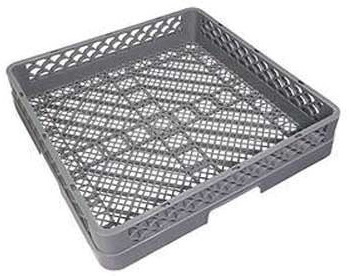
\includegraphics[height=6cm]{images/tray.jpg}
                \caption{Commercial Dishwashing Tray}\label{fig:tray}
            \end{figure}

            A gentry robot may be implemented to pick up the jars out of the tray to move them. The advantage of this style of robot is it is versatile and robust in it's actions. It can move anywhere within a predefined space, enough to encompass the entire tray and the conveyor ingress. The gantry is only a system of actuators and control systems, it still requires a subsystem to target where the jars are and thus where to move the end effector. 
            
            A camera may be implemented as a vision system for jar targeting. This can be used to sense the location of each jar present waiting to be unloaded, and pass the coordinates to the gantry robot.

        \subsection{Project Limitations}\label{sec:proj-limits}
            % needs to be on a rpi0. output meaningful for a targeting system.
            As per the project description, the processer hardware used must be a Raspberry Pi Zero W (hereafter ``Rpi''). This is single-board computer uses an ARMv6 architecture with a single-core CPU and no GPU. There is one available USB OTG connection. It has available and accessible GPIO and power pins. There is a connection for a CSI camera\cite{rpi}. 

            It was indicated in lecture that projects should include data collection via sensors connected to the Rpi as well as constructing the models. This greatly increases the project scope. Very large datasets are available  from open online sources. By using existing datasets, groups could have yielded interesting projects without needing to divert effort to anything other than than creating the models.
            
            % TODO any other limitations? specific issue will be discussed later in methodology

        \subsection{Design Philosophy}
            As we are currently training as Mechatronic Systems Engineers, we opted to take a holistic system based approach. This meant splitting the project in discrete subsystems and focusing on the integrations between systems, including subsystems before and after the scope of this project. This allowed us to create a project which was easily integrated into the existing industrial system and process. 

            It was decided that data collection will be a crucial step in this project. Without a sufficient dataset to train with, no matter the quality of the model, the results will be poor. Garbage in, garbage out. Great effort was put into data collection and labelling.

            \textbf{Input}: An unencoded image from a camera of the jars in a tray.

            \textbf{Output}: A list of coordinates, a spatial map of jar locations, or a single jar's coordinates. %TODO keep whichever it is

    \FloatBarrier
    \section{Methodology}
        \subsection{Data Collection}
            The data collection and labelling was all done manually. A series of photos of jars in different configurations in a tray were taken and saved. Between each photo, one jar would be altered. Once Sufficient photos were taken, each would be manually labelled using a custom made GUI. The images and labels would then be stored in a database for use by a model in training.

            \subsubsection{Camera Frame}
                % physical frame the camera and pi are mounted on
                A physical frame was constructed from wood and spare parts which holds the Rpi and camera in a fixed location over the jars and tray. A picture may be seen in figure~\ref{fig:frame}. The red part on the arm is the Rpi and camera. This allowed pictures to be taken of a consistent angle containing the same proportion of the tray every time. If the photos were taken from different angles each time, there would be too many variables introduced. Doing this minimized the number of features the model would need to compute. The frame worked well and as intended.

                \begin{figure}[ht]
                    \centering
                    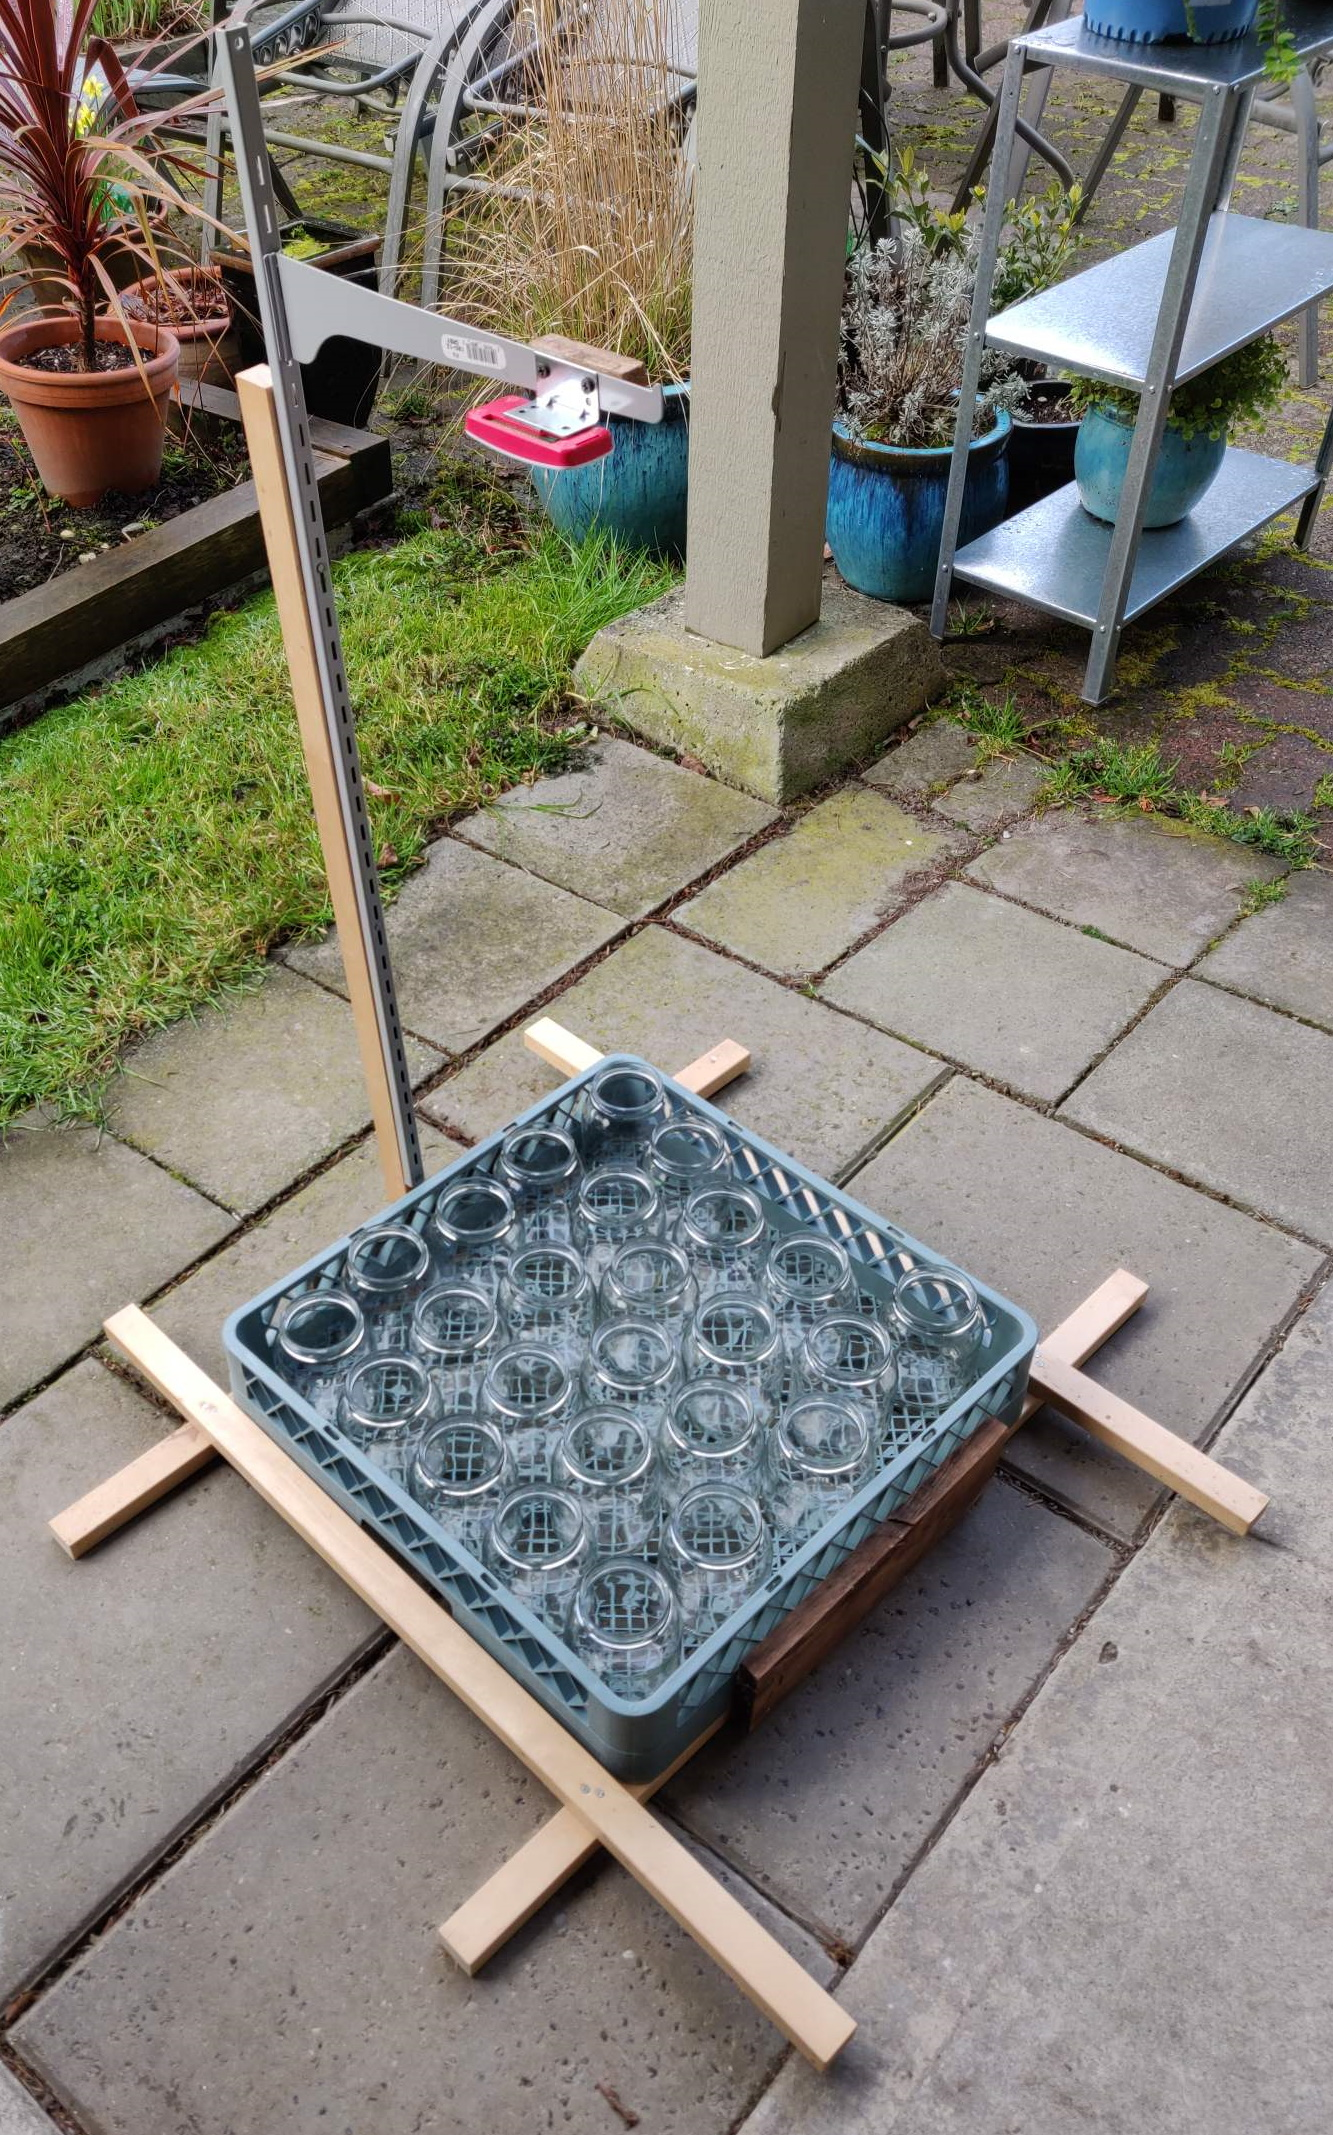
\includegraphics[height=9cm]{images/frame.jpg}      %TODO replace with better image
                    \caption{The Camera Mounting Frame}\label{fig:frame}
                \end{figure}

                The top-down perspective worked to mitigate the perspective warping from the camera lens. It will not be solved without a software transformation layer or the use of a different lens. It was decided that the perspective warping was outside the scope of this project.

            \subsubsection{Data Point Labelling}
                % taking photos and the GUI program
                To label the sizable collection of images collected with descript and precise coordinates, a program with a GUI was created. This program allowed fast labelling. A screenshot of this program may be seen in figure~\ref{fig:label-gui}. This program was exceedingly useful and greatly improved the data collection speed.

                % TODO
                \begin{figure}[ht]
                    \centering
                    
\includegraphics[height=9cm]{images/TODO.png}
                    \caption{The labelling program interface}\label{fig:label-gui}
                \end{figure}

                The interface was created with MatPlotLib, a graphing and visualization library for Python. To summarize how to use it, the user clicks on three points of the rim of a jar. Using equations~\ref{eq:x_0} through~\ref{eq:r}, the centre and radius is determined mathematically. A full user guide is present on the readme of the GitHub page. \(M_{i,j}\) is the \((i,j)\) minor from linear algebra. 

                \begin{align}
                    x_0 &= \frac{1}{2} \cdot \frac{M_{1,2}}{M_{1,1}} \label{eq:x_0}\\
                    y_0 &= -\frac{1}{2} \cdot \frac{M_{1,2}}{M_{1,1}} \label{eq:y_0}\\
                    r   &= x_0^2 + y_0^2 + \frac{M_{1,4}}{M_{1,1}} \label{eq:r}
                \end{align}

                There were issue in development with blocking inputs, sending interrupts from the buttons, and a memory leak. All of which were solved. After the images were labelled, the image, labels, and other information would be stored in a database.

            \subsubsection{Database}
                % storing all the data points
                Given that our training data is images, the dataset had the potential to require massive amounts of storage and the surrounding infrastructure. Implementing a MySQL database was considered but opted against. The work required to initialise the container, expose it safely for us both work with it, and the additional learning required to integrate it with Python was deemed too great for the minimal benefits at our prospective scale. This would be a more future-proof solution, but was excessive for our use.

                What was used was simple a list of dictionaries pickled then compressed into several archive files. This is a normal means of small-scale data storage in Python. This gave us to advantages of each data point having several different types of data, all listed under their respective key. Using multiple archive files allowed pushing/uploading them to GitHub with only free accounts. Each data point contained the unencoded RGB image, a list of jar centre coordinates, the filename of the origonal
                
                Several compression methods were experimented with. Of those, Lempel–Ziv–Markov chain algorithm (LZMA) was found to preform the fastest. bzip2 was, unexpectedly, found to have the greatest compression, roughly 25\% better than LZMA but was slightly slower. Deflate was found to have no benefits over LZMA or bzip2. bzip2 was chosen because the speed was still acceptable along with the better compression.

        \subsection{Machine Learning Model}
            % the Keras and other ML stuff
            \subsubsection{Data Augmentation} % maybe this should be in data collection
                % bolstering the data set with image transformations 

            \subsubsection{Keras Model Layers}
                % describing each layer in the model

        \subsection{Project Implementation and Integration}
            % how we got it to run on our hardware and how it will be integrated with the next subsystem
            \subsubsection{Tensor Flow on the Raspberry Pi}
                % how it got installed on armv6 and the tflite model exporting/importing

            \subsubsection{Raspberry Pi Program}
                % the program which executes on the pi. uses a pi camera to take and store photos for training. invokes the model when in use. full command line control possible.

            \subsubsection{Deriving Meaningful Data from the Model}
                % I don't know this yet

    \FloatBarrier
    \section{Results}
        \subsection{Example Results}
            % pictures visualizing the output of sample data

        \subsection{Results Metrics}
            % measurements quantifying the results
    
    \FloatBarrier
    \section{Discussions}
        % lots of graphs

    \FloatBarrier
    \section{Conclusion}

    \FloatBarrier
    \appendix
    
	\bibliographystyle{ieeetr}
	\bibliography{bib}\addcontentsline{toc}{section}{Referances}

	\section{List of Figures}
		\makeatletter
		\@starttoc{lof}% Print List of Figures
		\makeatother

	\section{List of Tables}
		\makeatletter
		\@starttoc{lot}% Print List of Tables
		\makeatother

\end{document}
